\section{Latency Calculation Algorithms}
\subsection{Key Concept}
When packets are transmitted from RAN, the timestamp when the packet is forwarded is stored for the outgoing packet. When the response for the packet arrives at the receiving side of RAN, the difference in time values of the current time and the stored timestamp  is calculated and then reported in the log file.
\subsubsection{Storing of Timestamp}
\begin{itemize}
	\item \textbf{Data Plane} The packet identification field in the IP header is used to identify the packet. These latency packets
	      are sent from the core CORE\_RTT. All the established sessions/UEs are used for forwarding the traffic. When the packet is
	      transmitted, a callback  function stores the outgoing packet timestamp in a hashmap with packet id as the key. This field is
	      generally used in the fragmentation and reassembly of packet data. The data plane latency packet throughput is substantially reduced by introducing sleep commands. The option of disabling the calculation of latency is removed as latency packets do not significantly affect any other metrics. Data plane latency is independently logged in a different column in the log file.
	\item \textbf{Control Plane}
	      This requires deep packet inspection of control plane packets. These packets are sent from the core CORE\_CP\_TRAFFIC.
	      There are three types of control plane packets - session establishment, session modification and session release packets - all of
	      them are used for measuring control plane latency. These packets have session ids stored at
	      different offsets in the payload.

	      Earlier, a hash map was used for storing the timestamps. The use of hashmap slows down the call backs and unnecessary limits the rate of data forwarding.

	      Subsequently, fixed length array was used to store timestamps - \textbf{TSArray} . The
	      array size is $65536 * 3$ and stores the value of timestamp register \textbf{rdtsc} of the
	      outgoing packets. The first $65536$ values are used to store establishment packet related
	      timestamps, next $65536$ modification packet related timestamps and then release packet
	      timestamps are stored.
	      The bitwise operations can be easily used as 65536 is a power of 2.


	      A callback function is registered on  the transmit queue corresponding to CORE\_CP\_TRAFFIC which stores the timestamp in the hashmap.
\end{itemize}
\subsection{Calculation of Latency}
A single callback function is registered on the CORE\_RX\_POLL which  receives the incoming packet.
\begin{itemize}
	\item \textbf{Data Plane} The same outgoing packet is reflected by the DNN packet and stored timestamp is retrieved from the hashmap and the difference is the end to end latency of each packet.
	\item \textbf{Control Plane} Every control plane packet has a response packet - establishment response (51), modification response (53), release response (55). The control plane latency is the time period from when the request packet is sent and the response packet is received.
	      The response packets have message type and either session IDs in their payload. For
	      modification and deletion  responses, the session ids have a difference of 3000.  Using these information, the index in \textbf{TSArray} can be calculated and the corresponding timestamp can be retrieved.
\end{itemize}
\subsection{Why do we need different techniques for control plane and data plane?}
\begin{itemize}
	\item \textbf{Why can't we use packet identifier for control plane packets?}
	      Both types of packets are received on the same rx queue/core. So, only the packet identifier in ip header is not enough to differentiate control plane and data plane packets. And you will need deep packet inspection to differentiate among the two packets.
	\item \textbf{Why don't we inspect packet payload for data plane packets?} Data plane packet has no useful payload and when the ip header identification field is unused till now, we can use it.
	\item \textbf{Development Sequence}
	      Data plane latency was implemented earlier when the packet id field was unused. Control plane latency calculation is done later.
\end{itemize}

\section{Callback functions}
Call back functions are registered on receive and transmit queues for latency calculation.
\begin{itemize}
	\item \textbf{CPStoreTimestampCallback}
	      Registered on CORE\_CP\_TRAFFIC for storing the timestamp of outgoing control plane packets.
	\item \textbf{DPStoreTimestampCallback}
	      Registered on CORE\_RTT for storing the timestamp of outgoing  data plane latency packets.

	\item \textbf{CPLatencyCallback}
	      Registered on CORE\_RX\_POLL for inspecting responses to control plane
	      requests. The difference in the current time and the  timestamp stored during the
	      tx callbacks gives the latency values.
	\item \textbf{DPLatencyCallback}
	      Also registered on CORE\_RX\_POLL for inspecting the mirrored data plane
	      latency packets.
\end{itemize}
%Run-to-Completion and Pipeline are two models of execution for packet processing and forwarding at User Plane Function.
%Comparison of these models in the different use cases/scenarios is one of the major objectives of our work. This chapter will explain these models of execution.
%
%\section{Run-to-Completion (RTC) \label{secRTC} }
% \begin{figure}[htbp]
%    \centering
%    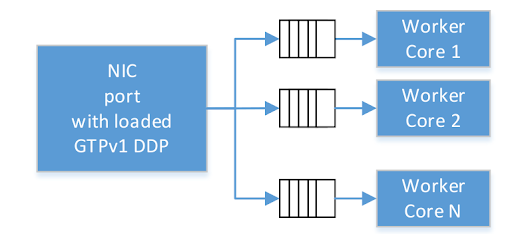
\includegraphics[width=0.7\textwidth, keepaspectratio]{./fig/ModelsofExecution/RTC.png}
%    \caption{Run-to-Completion}
%    \label{figRTC}
%    \end{figure}
%Keeping processors independent with minimal or no communication between them is the key idea of this model. Each
% processor should be able to completely recieve, process and forward/transmit the packet if required. Redirection of packets on different core requires receive side scaling (RSS) discussed in chapter \ref{chapterRSS}. Packets of a session are redirected to the same core as RSS value for packets of the same session is same.
%\section{Pipeline \label{secPipeline}}
%\begin{figure}[htbp]
%    \centering
%    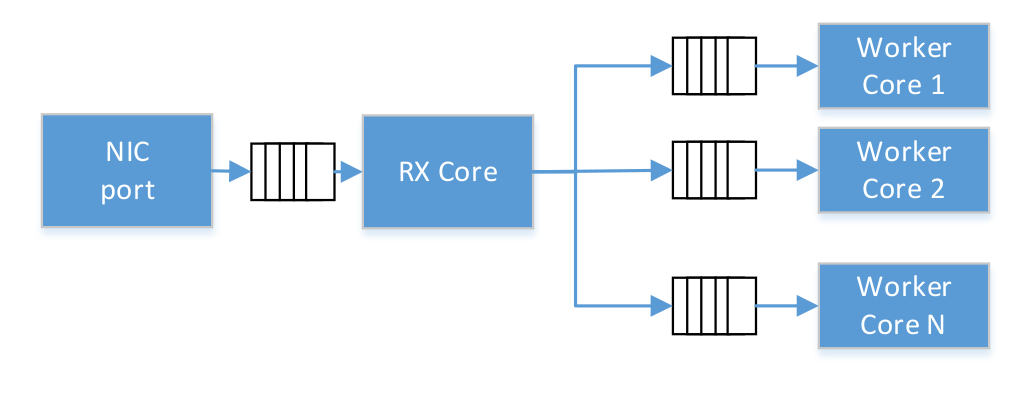
\includegraphics[width=0.7\textwidth, keepaspectratio]{./fig/ModelsofExecution/Pipeline.png}
%    \caption{Pipeline}
%    \label{figPipeline}
%\end{figure}
% Hardware based redirection is either not possible or not used in this model. Complete packet processing including redirection occurs in software. Packets are redirected to a master core which processes the outer headers to redirect packet on one of the worker cores. Generally packets of a session are redirected to the same core to maintain better spatial and temporal locality. However packets may be redistributed if a particular core gets overloaded.
%It requires inter-core communication. This communication happens through a software ring/circular queue for each worker core. The master core keeps incoming packets on the corresponding software ring of the worker core. The processed packets are then received by master core (through another ring) to transmit them over the wire.
%The pipeline model can also redistribute load by shifting load from high load core to least loaded loead.
%Our pipeline implementation handles this by mapping UEs from heavy loaded core to lightly loaded core. The UEs are remapped as long as there is no uniform distribution of load among different cores.
%\section{Comparison \label{RTCpipelineComparison}}
%
%The RTC has some significant advantages over the pipeline model.
%\begin{itemize}
%    \item \textbf{Better Throughput} The per core processing capability is expected to be higher in RTC model. This is due to no inter core communication and
% hardware support for hash computation. The computation in the hardware is generally faster than in software. This also keeps
%  CPUs meant for hash computation free for other tasks. 
%  \item \textbf{Lower Latency}The end to end latency in pipeline also takes a hit due to intercore
%   communication between master and worker core.
%\item \textbf{Easy to implement and understand} The RTC implementation's source code is easy to understand as it is same on all the cores. Pipeline has different logic and complex interaction between master and worker cores.
%\end{itemize}
% 
%However, pipeline is better suited to change operational behavior dynamically. This hypothesis is tested for two use cases.
%\begin{itemize}
%    \item \textbf{Dynamic Scaling} The key idea here is to start user plane function with minimum number of cores and vary
%     the number of cores according to the current traffic load. This helps in better energy efficiency as the cores may
%      remain idle when there is less traffic. It  is easy to reconfigure the number of cores in pipeline than RTC. RTC
%       requires stopping of ports before reconfiguring them as the number of RSS queues needs to be updated in hardware. A large number of packets are dropped during this reconfiguration. Pipeline requires the launch of cores in software which is relatively light weight.
%    \item \textbf{Redistribution of traffic}  Once flows are mapped to cores by hash output in RTC, it is not possible to redirect them to another core. This may be required when the load is
%     highly skewed towards some cores and the rest of the cores are idle. In such cases, a large number of packets are
%      dropped by heavily loaded core in RTC model. 
%    Pipeline can effectively handle such scenarios by redirecting certain flows from heavily loaded cores to less loaded cores. This reduces the number of packets dropped and better core utilisation. 
%\end{itemize}
%
%Experiments (discussed in chapter \ref{chapterExperimentsandResults}) were performed to test and evaluate these claims in 5G use case context. 
%